\documentclass[11pt,a4paper]{article}
\usepackage[T1]{fontenc}
\usepackage{lmodern}
\usepackage[margin=2.5cm]{geometry}
\usepackage{amsmath,amssymb}
\usepackage{graphicx}
\usepackage{booktabs}
\usepackage{multirow}
\usepackage{caption}
\usepackage[authoryear,round]{natbib}
\usepackage[hidelinks]{hyperref}
\usepackage{setspace}
\onehalfspacing
\captionsetup{font=small,labelfont=bf}

\title{Nonlinear dependence without low-dimensional chaos:\\[2pt]
\large a surrogate-based study of returns and volatility in ten cryptocurrencies and the Nifty 50 constituents}
\author{Anuj Kothari}
\date{Working draft, November 2026}

\begin{document}
\maketitle

\begin{abstract}
\noindent
Whether financial prices are generated by low-dimensional deterministic chaos has been asked repeatedly since the
late 1980s, and the answer has depended heavily on the null hypothesis against which chaos diagnostics are
judged. We revisit the question with a uniform, pre-specified protocol applied to 61 daily series: the ten largest
cryptocurrencies, the fifty current constituents of the Nifty 50 index and the index itself. For each asset we
study log returns, absolute returns, squared returns and 20-day realised volatility, and compute delay-embedding
parameters, the largest Lyapunov exponent, the correlation dimension, the 0--1 test for chaos, nonlinear
prediction skill, S-map nonlinearity gain and time-reversal asymmetry. Every statistic is compared with 999
iterative amplitude-adjusted Fourier transform (IAAFT) surrogates and 999 surrogates simulated from a fitted
GARCH(1,1) model with Student-$t$ innovations, with false discovery rate control within and across assets. We
complement the time-domain analysis with Welch power spectra, spectral exponents and band shares, tested against
the same surrogate families over the full sample and four market periods. The conventional chaos indicators are
uninformative on their own: the largest Lyapunov exponent is positive in 243 of 244 series, the correlation
dimension appears to saturate in most series and the 0--1 statistic is close to one everywhere, yet GARCH
surrogates reproduce all three. Nonlinear structure relative to a linear Gaussian null is widespread (all ten
cryptocurrencies and 42 of 51 Nifty series in returns), but after cross-asset correction only 2 of 1,464 tests
against GARCH remain significant, both isolated correlation-dimension results. No series is classified as
potentially chaotic. The one robust feature that GARCH does not reproduce is a seven-day spectral peak in the
absolute returns of every cryptocurrency (and in realised volatility of five), which we interpret as a weekly calendar effect rather than as deterministic
dynamics. The spectral shape of volatility also differs systematically between markets: relative to GARCH,
cryptocurrency volatility is less persistent, and squared returns of about a third of the stocks carry
more low-frequency power.

\medskip
\noindent\textbf{Keywords:} deterministic chaos; surrogate data; nonlinearity; GARCH; power spectrum;
cryptocurrencies; Nifty 50; multiple testing
\end{abstract}

% ------------------------------------------------------------------------------------------------------------
\section{Introduction}

The possibility that the irregular behaviour of asset prices reflects low-dimensional deterministic dynamics,
rather than the accumulation of exogenous random shocks, has attracted economists and physicists for more than
three decades. The appeal is easy to understand. A deterministic system with a small number of effective degrees of
freedom would be predictable over short horizons even if it looked random to linear methods, and theoretical
asset-pricing models with heterogeneous, boundedly rational traders can produce exactly such dynamics
\citep{BrockHommes1998}. The empirical literature that followed, however, taught a sobering lesson: the standard
diagnostics of chaos, namely a positive largest Lyapunov exponent, a low and saturating correlation dimension and
apparent structure in reconstructed phase space, can all be produced by stochastic processes, particularly by
processes with heavy tails, strong persistence or time-varying volatility
\citep{OsborneProvenzale1989,Ruelle1990,EckmannRuelle1992}. When the same diagnostics are applied to residuals of
models that capture conditional heteroskedasticity, most evidence for chaos in stock, currency and commodity
returns disappears \citep{Hsieh1989,Hsieh1991,BrockHsiehLeBaron1991}.

Two developments make the question worth revisiting. The first is methodological. Surrogate data testing
\citep{Theiler1992,SchreiberSchmitz1996,SchreiberSchmitz2000,Lancaster2018} and the 0--1 test for chaos
\citep{GottwaldMelbourne2004,GottwaldMelbourne2009} are now mature, and modern computing makes it possible to
use several hundred surrogates per test, for many statistics, many series and many assets, which in turn makes
proper control of the false discovery rate both possible and necessary \citep{BenjaminiHochberg1995,Harvey2016}.
The second is the emergence of cryptocurrency markets, which trade continuously, are dominated by retail and
algorithmic participants, and display volatility and tail behaviour far more extreme than those of equity
markets \citep{Corbet2019}. Several studies report chaos or strong nonlinear structure in Bitcoin
\citep{LahmiriBekiros2018}, but such conclusions typically rest on comparisons with linear or independent null
models, which are known to be rejected by any series with volatility clustering.

This paper asks a deliberately narrow question: once the stylised facts of returns, namely heavy tails and
volatility clustering, are respected by the null model, is there evidence of low-dimensional deterministic
dynamics, or of any nonlinear structure beyond a standard volatility model, in daily returns and volatility of
cryptocurrencies and of large Indian stocks? We make three contributions.
\begin{enumerate}
\item We apply a single, pre-specified protocol to 61 assets from two very different markets and four
transformations of each return series, so that results are comparable across assets and are not the product of
asset-by-asset tuning. The protocol combines geometric diagnostics (embedding, Lyapunov exponent, correlation
dimension), a dynamical diagnostic (the 0--1 test), predictive diagnostics (simplex and S-map) and a symmetry
diagnostic (time reversal).
\item Every statistic is judged against two surrogate families with different null hypotheses: IAAFT surrogates,
which preserve the linear autocorrelation and the marginal distribution, and GARCH(1,1)-$t$ surrogates, which
additionally reproduce volatility clustering and heavy tails. Results are corrected for multiple testing both
within each asset and across all assets, and checked for stability in the two halves of each sample.
\item We add a frequency-domain analysis that is usually absent from chaos studies in finance: Welch power
spectra, spectral exponents and band shares, compared with surrogate spectra over the full sample and over four
market periods. This turns out to be where the only robust departure from the GARCH null appears.
\end{enumerate}

The results are negative regarding chaos and informative regarding everything else. The classical diagnostics
look ``chaotic'' in almost every series, but GARCH surrogates look equally chaotic. Nonlinearity relative to a
linear null is pervasive, but it is almost entirely accounted for by conditional heteroskedasticity. No series is
classified as potentially chaotic. What survives is a weekly cycle in cryptocurrency volatility and systematic
differences between the two markets in the spectral shape of volatility, both of which point to calendar and
persistence effects that a GARCH(1,1) model omits rather than to deterministic dynamics.

Section~\ref{sec:lit} reviews the literature. Section~\ref{sec:data} describes the data,
Section~\ref{sec:method} the methods and Section~\ref{sec:results} the results. Section~\ref{sec:discussion}
discusses the interpretation, and Section~\ref{sec:conclusion} concludes.

% ------------------------------------------------------------------------------------------------------------
\section{Literature review}\label{sec:lit}

\subsection{From strange attractors to time-series diagnostics}

The empirical study of chaos in observed data rests on the embedding theorem of \citet{Takens1981}, generalised
by \citet{Sauer1991}: for a deterministic system whose trajectories lie on an attractor of dimension $D$, a vector
of $m$ delayed observations $(x_t, x_{t-\tau},\dots,x_{t-(m-1)\tau})$ with $m > 2D$ generically reconstructs the
attractor up to a smooth change of coordinates. Practical reconstruction requires choosing the delay $\tau$ and
the dimension $m$. The delay is commonly taken at the first minimum of the average mutual information
\citep{FraserSwinney1986} or where the autocorrelation function has decayed sufficiently, and the dimension is the
smallest $m$ at which the fraction of false nearest neighbours vanishes \citep{Kennel1992}. Invariants of the
reconstructed attractor then characterise the dynamics: the correlation dimension of \citet{GrassbergerProcaccia1983},
estimated from the scaling of the correlation sum, and the largest Lyapunov exponent, estimated from the average
exponential divergence of initially close trajectories \citep{Wolf1985,Rosenstein1993}. Comprehensive treatments
are given by \citet{EckmannRuelle1985} and \citet{KantzSchreiber2004}. Recurrence plots
\citep{Eckmann1987} and recurrence quantification \citep{Marwan2007} provide visual and quantitative summaries of
recurrences in phase space.

A different route to detecting chaos avoids phase-space reconstruction altogether. \citet{GottwaldMelbourne2004}
proposed the 0--1 test, which drives a two-dimensional system with the observed series and measures whether the
resulting trajectory is bounded (regular dynamics, $K \approx 0$) or diffusive (chaotic dynamics, $K\approx 1$);
implementation issues such as oversampling and the choice of frequency are discussed in
\citet{GottwaldMelbourne2009}. A third route uses prediction. \citet{SugiharaMay1990} showed that for chaotic
systems the skill of nearest-neighbour (simplex) forecasts declines with horizon, whereas for uncorrelated noise it
is flat, and \citet{Sugihara1994} introduced the S-map, a locally weighted linear forecast whose improvement over a
global linear model as the locality parameter increases measures state-dependent, that is nonlinear, dynamics.

\subsection{The critique: stochastic processes that look chaotic}

The early enthusiasm for these diagnostics was tempered by a series of results showing how easily they are
misled. \citet{Theiler1986} showed that temporal correlation produces spurious low correlation dimensions unless
temporally close points are excluded. \citet{OsborneProvenzale1989} showed that coloured stochastic processes with
power-law spectra have finite, saturating correlation dimensions. \citet{Ruelle1990} and \citet{EckmannRuelle1992}
derived the data requirements for meaningful dimension and Lyapunov estimates, which grow exponentially with the
dimension and are rarely met by economic time series. The Rosenstein divergence curve has a positive initial slope
for many noisy stochastic series, so a positive estimated exponent is a necessary but not a sufficient sign of
chaos; and the 0--1 test returns $K\approx 1$ for uncorrelated noise as well as for chaos, so it cannot by itself
distinguish the two \citep{GottwaldMelbourne2009}.

The constructive response to these problems was the method of surrogate data \citep{Theiler1992}. A null
hypothesis is specified as a class of processes, an ensemble of artificial series consistent with the null is
generated from the data, and the discriminating statistic computed on the data is ranked within its distribution
over the surrogates. Amplitude-adjusted Fourier transform surrogates test the null of a linear Gaussian process
observed through a static monotone transformation; the iterative refinement of \citet{SchreiberSchmitz1996}
matches the power spectrum and the marginal distribution more accurately. \citet{SchreiberSchmitz2000} and
\citet{Lancaster2018} review surrogate methods and warn that rejection of a linear null says only that the series is
not linear Gaussian; it does not say what it is. In financial data, where volatility clustering guarantees
rejection of linear nulls, model-based surrogates that preserve conditional heteroskedasticity are the natural
next step. Time-reversal asymmetry provides a complementary, model-free signature: linear Gaussian processes and
their static transforms are statistically reversible, so asymmetry indicates nonlinearity or non-Gaussian driving
\citep{Diks1995,RamseyRothman1996}.

\subsection{Chaos and nonlinearity in financial markets}

Applications to financial data began in the late 1980s. \citet{ScheinkmanLeBaron1989} found that the correlation
dimension of weekly US stock returns was lower than that of shuffled returns, and proposed the comparison with
shuffled data that underlies the BDS test \citep{BDS1996}. \citet{FrankStengos1989} reported low dimensions for gold
and silver returns, and \citet{Peters1991} popularised chaos and fractal ideas in the practitioner literature.
The decisive counter-evidence came from studies that applied the same tests to standardised residuals of GARCH-type
models: \citet{Hsieh1989} for exchange rates and \citet{Hsieh1991} for stock returns found that nonlinear dependence
is largely explained by conditional heteroskedasticity and found no convincing evidence of chaos, a conclusion
summarised in the monograph of \citet{BrockHsiehLeBaron1991}. \citet{MayfieldMizrach1992} estimated dimensions for
high-frequency S\&P 500 data and found them high, and \citet{Abhyankar1997} found nonlinear dependence but no
evidence of low-dimensional chaos in four major stock indexes at high frequency. \citet{BarnettSerletis2000}
reviewed the econometric evidence and concluded that tests for chaos in economic data are inconclusive at best and
that their power against realistic stochastic alternatives is poorly understood; \citet{KyrtsouSerletis2006}
reached similar conclusions with a battery of univariate tests. On the linearity side, tests such as those of
\citet{Hinich1982} and \citet{Tsay1986} routinely reject linearity in returns, consistent with the stylised facts
collected by \citet{Cont2001}: heavy tails \citep{Mandelbrot1963}, volatility clustering
\citep{Engle1982,Bollerslev1986,Bollerslev1987}, and slow decay of the autocorrelation of absolute returns
\citep{DingGrangerEngle1993}.

\subsection{Volatility persistence, long memory and the spectrum}

Spectral methods have a long history in economics; \citet{Granger1966} documented the ``typical spectral shape''
of economic variables, with power concentrated at low frequencies. For volatility, the slow, hyperbolic decay of
autocorrelations in absolute and squared returns \citep{DingGrangerEngle1993} corresponds to a spectrum that
diverges as a power law at low frequency, $S(f)\propto f^{-\beta}$ with $\beta = 2d$ for a fractionally integrated
process of order $d$. The memory parameter can be estimated semiparametrically from the low-frequency periodogram
\citep{GewekePorterHudak1983}, and long-memory volatility models such as FIGARCH \citep{Baillie1996} and the
heterogeneous autoregressive model of realised volatility \citep{Corsi2009,Andersen2003} were proposed to capture
it. At the same time, apparent long memory can be generated by structural breaks or slowly changing parameters in
short-memory models: \citet{LamoureuxLastrapes1990} showed that breaks inflate the estimated persistence of GARCH
models, and \citet{MikoschStarica2004} showed that nonstationarity can produce both apparent long-range dependence
and integrated GARCH estimates. \citet{Lo1991} showed that classical rescaled-range tests confuse short-range
dependence with long memory. Periodic components are also well known in volatility: \citet{AndersenBollerslev1997}
showed that intraday periodicity in volatility distorts estimates of volatility persistence if it is not removed.
These results are directly relevant to chaos testing, because a power-law spectrum or a persistent volatility
process is exactly the kind of stochastic structure that misleads dimension and Lyapunov estimates
\citep{OsborneProvenzale1989}. In the physics literature, offset log-scale spectra across regimes are a standard way
to compare dynamics between parameter ranges \citep[e.g.][]{KailashamKhair2023}; we borrow this presentation for
comparing market periods.

\subsection{Cryptocurrencies}

The cryptocurrency literature has focused on market efficiency, volatility modelling and calendar effects.
\citet{Urquhart2016} found that Bitcoin returns were inefficient in its early years and becoming more efficient
over time, and \citet{Bariviera2017} reached similar conclusions with time-varying Hurst exponents.
\citet{Katsiampa2017} compared GARCH specifications for Bitcoin and found that models with a long-run and a
short-run volatility component fit best. \citet{LahmiriBekiros2018} applied the largest Lyapunov exponent and
entropy measures to Bitcoin prices and reported chaos and multifractality, without model-based surrogates.
\citet{Corbet2019} survey the field. On calendar effects, the evidence is mixed for returns but clearer for activity
and volatility: \citet{Baur2019} found weekday and weekend differences in Bitcoin trading volume and volatility,
\citet{Caporale2019} found a day-of-the-week effect in Bitcoin returns but not in other coins, and
\citet{AharonQadan2019} reported day-of-the-week effects in both Bitcoin returns and volatility. In equity markets the
weekend effect in returns is a classic anomaly \citep{French1980}. To our knowledge, no previous study has linked
the weekly calendar structure of cryptocurrency volatility to the question of nonlinear or chaotic dynamics, or
shown that it is the main feature that a GARCH null fails to reproduce.

\subsection{Gap addressed by this paper}

Three gaps motivate the present study. First, most chaos studies of individual assets use a single null model,
often linear, so that rejection is guaranteed by volatility clustering and is easily over-interpreted. Second,
studies rarely apply the same protocol to many assets with control of the false discovery rate across assets,
although with dozens of statistics per series the expected number of false positives is substantial
\citep{BenjaminiHochberg1995,Harvey2016}. Third, frequency-domain evidence and time-domain chaos diagnostics are
rarely examined together, although the former explains many of the artefacts of the latter. Indian equities, despite
the size of the market, have received comparatively little attention in this literature, and a direct comparison of
a 24/7 cryptocurrency market with an exchange-traded equity market under one protocol is, as far as we know, new.

% ------------------------------------------------------------------------------------------------------------
\section{Data}\label{sec:data}

\paragraph{Cryptocurrencies.} We use daily closing prices (00:00 UTC) of the ten cryptocurrencies with the largest
trading volume at the time of download, quoted against the US dollar stablecoin USDT on a large spot exchange:
BTC, ETH, BNB, SOL, XRP, DOGE, ADA, AVAX, TRX and DOT. Each series starts on the first available trading day
(2017-09-06 for BTC and ETH; between 2017-11 and 2020-10 for the others) and ends on 2026-09-02. The number of daily
returns ranges from 2,152 (AVAX) to 3,284 (BTC, ETH), with a median of 3,005. Cryptocurrencies trade seven days a
week, so a ``day'' is a calendar day.

\paragraph{Nifty 50.} We use daily dividend- and split-adjusted closing prices of the fifty stocks in the Nifty 50
index at the time of download, and the closing level of the index itself, from 2016-01-01 to 2026-10-16. The price
panel was cleaned before this study: days on which nearly all stocks reported zero volume and unchanged prices were
removed, and two corporate actions not reflected in the source data were corrected. Most stocks have 2,644 daily
returns. Six were listed after 2016; the shortest histories are JIOFIN (758 returns) and ETERNAL (1,273 returns),
which we flag as ``low power'' (between 750 and 1,499 observations); every other asset has at least 1,500
observations. The constituent list is the current one, so the sample is subject to survivorship bias. The data were
read only and never modified.

\paragraph{Series analysed.} For each asset we compute log returns $r_t=\ln P_t-\ln P_{t-1}$ and four series:
returns $r_t$, absolute returns $|r_t|$, squared returns $r_t^2$, and 20-day realised volatility
$\mathrm{RV}_t=\big(\tfrac{1}{20}\sum_{j=0}^{19} r_{t-j}^2\big)^{1/2}$. The first 19 observations are dropped from all
four series so that they are aligned. Daily return volatility is very different in the two markets: the median
(across assets) standard deviation of daily returns is 0.051 for cryptocurrencies and 0.018 for Nifty stocks.

\paragraph{Market periods.} For the period analysis we split each sample into four periods chosen before the
analysis to separate broad market regimes: P1 (2017-09 to 2019 for crypto, 2016--2019 for Nifty), P2 (2020--2021,
including the COVID-19 crash and the 2021 boom), P3 (2022--2023) and P4 (2024 to the end of the sample). A period is
analysed for an asset only if the asset has at least 365 observations in it and at least half of the nominal period;
this gives 6, 10, 10 and 10 cryptocurrencies and 48, 48, 50 and 51 Nifty series in P1 to P4.

% ------------------------------------------------------------------------------------------------------------
\section{Methods}\label{sec:method}

All settings below were fixed before the cross-asset run and are identical for every asset. The pseudo-random
generator is seeded deterministically for every surrogate, so all results are exactly reproducible.

\subsection{Embedding}
Each series is standardised. The delay $\tau$ is the smaller of the first local minimum of the average mutual
information (16 equiprobable bins, lags up to 30) and the first lag at which the absolute autocorrelation falls below
$1/e$. The embedding dimension $m$ is the smallest $m\le 10$ at which the fraction of false nearest neighbours
\citep{Kennel1992} falls below 5\%; if no such $m$ exists, $m=10$ is used and the series is recorded as not having
reached a low-dimensional embedding. Temporally close neighbours are excluded with a Theiler window of
$\max(10, 2\tau)$ observations, and at least 20 for realised volatility, whose overlapping construction induces 20
days of mechanical dependence.

\subsection{Chaos diagnostics}
\begin{itemize}
\item \emph{Largest Lyapunov exponent} (LLE): the algorithm of \citet{Rosenstein1993}, with the slope of the mean
log-divergence curve fitted from step 1 to the first step at which the curve has completed 60\% of its total rise
(at least four steps). The goodness of the linear fit is recorded.
\item \emph{Correlation dimension} $D_2$: correlation sums with the maximum norm on up to 2,000 embedded points
\citep{GrassbergerProcaccia1983}, local slopes in the scaling range $10^{-3}\le C(r)\le 10^{-1}$, for $m=1,\dots,10$.
We say that $D_2$ saturates if some three consecutive values of $m$ have slopes within 15\% of their mean and that
mean is below $m-1$. This rule was validated on the logistic map before use. For surrogate testing, the
statistic is the slope at $m=5$.
\item \emph{0--1 test}: the correlation method of \citet{GottwaldMelbourne2009} applied to the series subsampled
every $\tau$ steps, with the median $K$ over 50 random frequencies $c\in(\pi/5,4\pi/5)$.
\item \emph{Recurrence determinism} (DET): the share of recurrence points on diagonal lines of length at least 2,
for the last 1,000 embedded points at a 10\% recurrence rate. DET is reported descriptively only.
\end{itemize}

\subsection{Nonlinearity diagnostics}
\begin{itemize}
\item \emph{Prediction skill}: the out-of-sample correlation between one-step simplex forecasts \citep{SugiharaMay1990}
and outcomes, with the first 70\% of the sample as library.
\item \emph{S-map gain}: $1-\mathrm{MSE}_{\theta^*}/\mathrm{MSE}_{0}$, where $\mathrm{MSE}_0$ is the one-step error
of a global linear autoregression on the embedding vector and $\mathrm{MSE}_{\theta^*}$ is the smallest error of the
S-map \citep{Sugihara1994} for $\theta\in\{1,2,4\}$, both evaluated on the last part of the sample.
\item \emph{Time-reversal asymmetry}: $\langle (x_{t+1}-x_t)^3\rangle/\langle (x_{t+1}-x_t)^2\rangle^{3/2}$, which
is zero in expectation for reversible processes \citep{Diks1995,RamseyRothman1996}.
\end{itemize}

\subsection{Surrogates and hypothesis tests}
Two surrogate families are used, each with 999 members per series.
\begin{enumerate}
\item \emph{IAAFT} \citep{SchreiberSchmitz1996}: 200 iterations, generated directly from each of the four series.
The null hypothesis is a stationary linear Gaussian process observed through a static monotone transformation.
\item \emph{GARCH(1,1)-$t$}: a GARCH(1,1) model with constant mean and Student-$t$ innovations
\citep{Bollerslev1986,Bollerslev1987} is fitted by maximum likelihood to the returns of each asset; return paths of
the same length are simulated (500 burn-in steps) and transformed into absolute returns, squared returns and
realised volatility exactly as the data are. The null hypothesis is that the series is generated by this
volatility model. It preserves heavy tails and volatility clustering but contains no deterministic dynamics.
\end{enumerate}
For each statistic the rank $p$-value is $(1+\#\{\text{surrogates at least as extreme}\})/(N+1)$, one-sided where the
direction is implied by the alternative (lower $D_2$, higher prediction skill, higher S-map gain) and two-sided
otherwise. With $N=999$ the smallest attainable $p$-value is 0.001 (one-sided) and 0.002 (two-sided). As an effect size we
report $z$, the difference between the observed statistic and the surrogate mean divided by the surrogate standard
deviation.

\paragraph{Multiple testing.} Each asset has $4\times 6\times 2=48$ surrogate tests. Within an asset they are adjusted
with the Benjamini--Hochberg procedure \citep{BenjaminiHochberg1995}. Across assets, the 61 $p$-values of each test
family (series $\times$ statistic $\times$ surrogate family) are adjusted together, and we call a result significant
across assets if its cross-asset $q$-value is below 0.05.

\paragraph{Split-sample stability.} The full set of tests is repeated on the first and second halves of each sample
with 499 surrogates per family and independent seeds.

\paragraph{Classification rule.} Each series is assigned to one class by a rule fixed in advance:
\emph{Periodic} or \emph{Quasi-periodic} if $K<0.2$ and $D_2$ saturates (distinguished by the value of $D_2$);
\emph{Potentially Chaotic} if $K>0.8$, $D_2$ saturates and at least two of the deterministic statistics ($D_2$,
prediction skill, S-map gain, LLE) are significant against \emph{both} surrogate families; \emph{Random/Stochastic} if
$K>0.8$ and no statistic is significant against GARCH; \emph{Inconclusive} otherwise. A positive LLE, a saturating
$D_2$ or a visual pattern alone never leads to a chaotic classification.

\subsection{Power spectra}
Spectra are estimated with Welch's method \citep{Welch1967} on the standardised series (Hann window, 512-day segments,
50\% overlap, linear detrending), giving a frequency resolution of $1/512$ cycles per day. We report:
(i) the spectral exponent $\beta$ from an ordinary least squares fit of $\log S$ on $\log f$ over periods of 25 to
250 days, with its $R^2$; (ii) the semiparametric estimate $\beta_{\mathrm{GPH}}=2\hat d$ of
\citet{GewekePorterHudak1983} using the lowest $\sqrt n$ Fourier frequencies; (iii) the shares of spectral power at
periods longer than 20 days (low band) and shorter than 5 days (high band); (iv) the three largest spectral peaks
with periods up to 250 days. Each quantity is compared with its distribution over 999 surrogate spectra of each
family. The whole spectrum is tested with a global maximum-deviation statistic,
$D=\max_f |\log S(f)-\mathrm{med}_0(f)|/\mathrm{sd}_0(f)$, computed identically for the data and each surrogate, which
controls the family-wise error over frequencies. A weekly component is tested one-sided at the Welch frequency
closest to one cycle per seven days for cryptocurrencies and one cycle per five trading days for stocks. This
frequency was specified in advance as a calendar check; the cross-asset analysis is therefore a replication of the
Bitcoin result, which was obtained first. Spectral $p$-values are adjusted within each asset and across assets in
the same way as the surrogate tests.

Two features of the spectra are mechanical and are taken into account in interpretation. The 20-day moving average
in realised volatility has spectral zeros at $f=k/20$ cycles per day, which appear as evenly spaced dips in its
spectrum; the GARCH surrogates pass through the same filter, so comparisons with them remain valid. One of these
zeros falls at $f=0.2$, the five-day frequency, so the weekly test for realised volatility of stocks is uninformative
by construction.

\subsection{Period analysis}
For each market period we compute time-domain summaries (mean, standard deviation, kurtosis, lag-1
autocorrelation) and Welch spectra with 256-day segments, the spectral exponent over periods of 25 to 128 days and
the band shares. Each period is compared with 499 GARCH surrogates of a model refitted to that period only, and with
499 IAAFT surrogates, using the global spectral test and tests on $\beta$ and the low-band share. Spectra of different
periods are displayed with vertical offsets on a logarithmic axis, following the presentation of
\citet{KailashamKhair2023}.

\subsection{Computation}
The full protocol requires about 40,000 surrogate series per asset. It was run on a shared workstation using at most
half of its processors, with each analysis stage checkpointed to disk. The Bitcoin results obtained on this machine
were checked against an independent run of the same code on a different computer and agree to the last reported
digit.

% ------------------------------------------------------------------------------------------------------------
\section{Results}\label{sec:results}

\subsection{Embedding and conventional chaos indicators}

Table~\ref{tab:diag} summarises the diagnostics across assets. Three observations stand out. First, no
low-dimensional embedding is found: for returns, absolute returns and realised volatility, the false-nearest-neighbour
fraction never falls below 5\% for $m\le 10$ in any of the 61 assets, and for squared returns it does so in only 3
cryptocurrencies and 5 Nifty series. The delay is one day for the return-based series and about 21 to 22 days for
realised volatility, where it reflects the averaging window. Second, the conventional indicators would, if taken at
face value, suggest chaos almost everywhere: the LLE is positive in 243 of 244 series, with median values between
0.07 and 0.20 per day; $D_2$ satisfies the saturation rule in 78\% to 100\% of series depending on the transformation,
at values between 2.5 and 5.5; and the 0--1 statistic $K$ lies between 0.97 and 1.00 in every series. Third, and
decisively, GARCH surrogates produce the same values. For returns, the median LLE is 0.114 in the cryptocurrency data
and 0.113 in their GARCH surrogates, and 0.113 against 0.113 for Nifty; the median $D_2$ at $m=5$ is 4.00 against
4.12 (crypto) and 4.26 against 4.33 (Nifty); and the median $K$ is 0.998 in both data and surrogates. A process with no
deterministic component at all thus reproduces every conventional ``signature of chaos'' in these data.

\begin{table}[t]
\centering
\small
\caption{Embedding and chaos diagnostics across assets (medians across assets unless stated). FNN: share of assets for
which the false-nearest-neighbour fraction reached 5\% at some $m\le 10$. LLE $>0$ and $D_2$ sat.: share of assets with
a positive Lyapunov exponent and a saturating correlation dimension.}
\label{tab:diag}
\begin{tabular}{llrrrrrrr}
\toprule
Market & Series & $\tau$ & FNN & LLE & LLE $>0$ & $D_2$ sat. & $D_2$ & $K$ \\
\midrule
\multirow{4}{*}{Crypto (10)} & returns & 1 & 0.00 & 0.114 & 1.00 & 1.00 & 4.51 & 0.997\\
 & absolute returns & 1 & 0.00 & 0.138 & 1.00 & 1.00 & 4.00 & 0.998\\
 & squared returns & 1 & 0.30 & 0.203 & 1.00 & 0.80 & 2.52 & 0.999\\
 & realised vol (20d) & 22 & 0.00 & 0.066 & 1.00 & 0.90 & 5.22 & 0.994\\
\midrule
\multirow{4}{*}{Nifty (51)} & returns & 1 & 0.00 & 0.113 & 1.00 & 0.94 & 5.49 & 0.998\\
 & absolute returns & 1 & 0.00 & 0.133 & 1.00 & 0.94 & 4.98 & 0.998\\
 & squared returns & 1 & 0.10 & 0.189 & 0.98 & 0.98 & 2.98 & 0.998\\
 & realised vol (20d) & 21 & 0.00 & 0.066 & 1.00 & 0.78 & 5.42 & 0.996\\
\bottomrule
\end{tabular}
\end{table}

\subsection{Nonlinearity relative to a linear null}

Against IAAFT surrogates, nonlinear structure is common (Figure~\ref{fig:share}, light bars). After cross-asset
correction, returns differ from their IAAFT surrogates in all ten cryptocurrencies and in 42 of 51 Nifty series;
absolute returns in 7 of 10 and 11 of 51; realised volatility in 6 of 10 and 5 of 51; squared returns in 1 of 10 and 5
of 51. In total 119 of 1,464 IAAFT tests are significant across assets. The statistic responsible is most often the
LLE of returns (all ten cryptocurrencies and 41 Nifty series), followed by the S-map gain of returns (3 and 13) and
time-reversal asymmetry in absolute returns and realised volatility. The sign of the LLE effect is informative: the
exponent of the data is \emph{smaller} than that of the IAAFT surrogates (median $z=-2.9$ for crypto, $-2.8$ for
Nifty), the opposite of what an additional chaotic component would produce. Time-reversal asymmetry of volatility has
opposite signs in the two markets: positive for every significant cryptocurrency series (median $z=4.3$ for absolute
returns and $10.4$ for realised volatility) and negative for most significant Nifty series.

\begin{figure}[t]
\centering
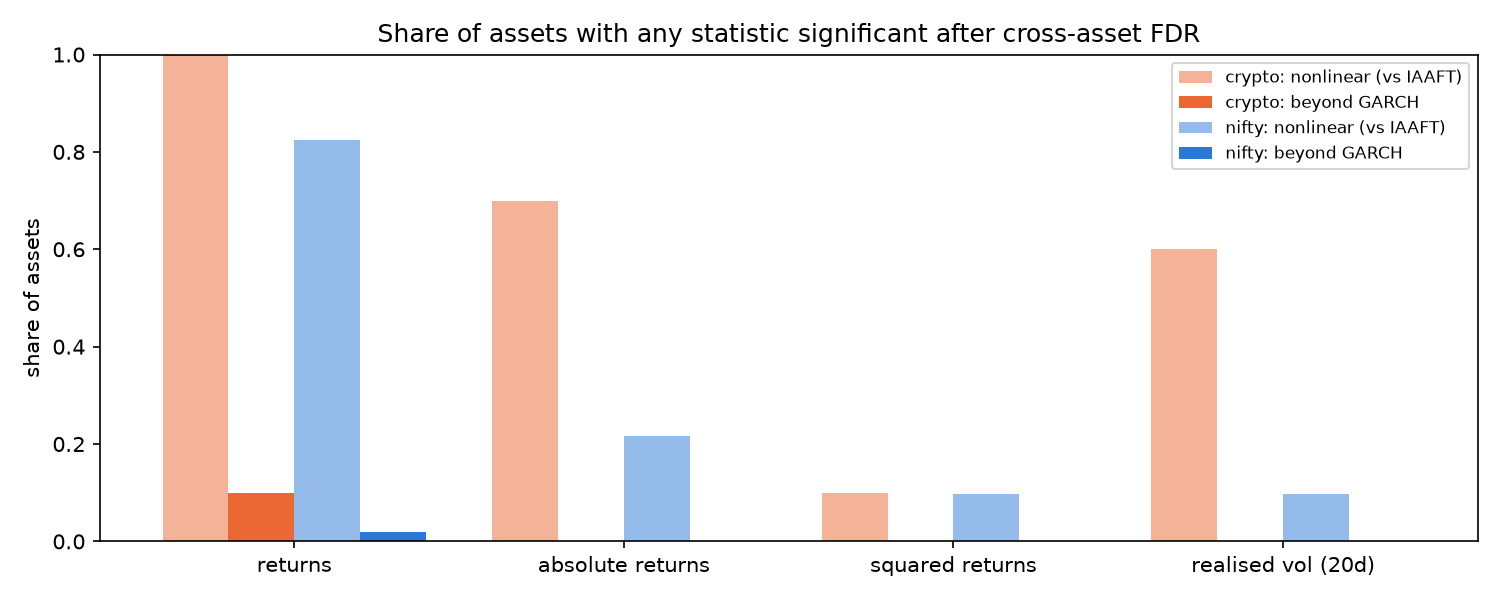
\includegraphics[width=0.85\textwidth]{figures/03_share_nonlinear_beyond_garch.png}
\caption{Share of assets in which at least one statistic is significant after cross-asset false discovery rate
control, by series and market. Light bars: against IAAFT surrogates (nonlinearity relative to a linear Gaussian
null). Dark bars: against GARCH(1,1)-$t$ surrogates.}
\label{fig:share}
\end{figure}

\subsection{Nonlinearity relative to the GARCH null}

Against GARCH surrogates the picture changes completely (Figure~\ref{fig:share}, dark bars, and
Figure~\ref{fig:heat}). Of the 1,464 tests against GARCH, two remain significant after cross-asset correction: the
correlation dimension of DOGE returns ($z=-4.5$, $q=0.03$) and of SBILIFE returns ($z=-3.1$, $q=0.03$). Neither is
accompanied by any other significant statistic in the same series, and neither replicates in the second half of its
sample. At the nominal 5\% level, 133 tests have $p\le 0.05$ against an expectation of 73 under the global null, so
there is a modest excess of small $p$-values, spread thinly across statistics and assets; the largest shares of
$|z|>1.96$ are in the S-map gain of absolute returns (20\% of assets), the LLE of realised volatility (18\%) and the
time-reversal asymmetry of squared returns (18\%). This pattern is what one would expect from a model that is
slightly misspecified in many small ways (for example in its tail shape, its asymmetry, or its persistence) rather
than from a strong common deterministic signal.

\begin{figure}[p]
\centering
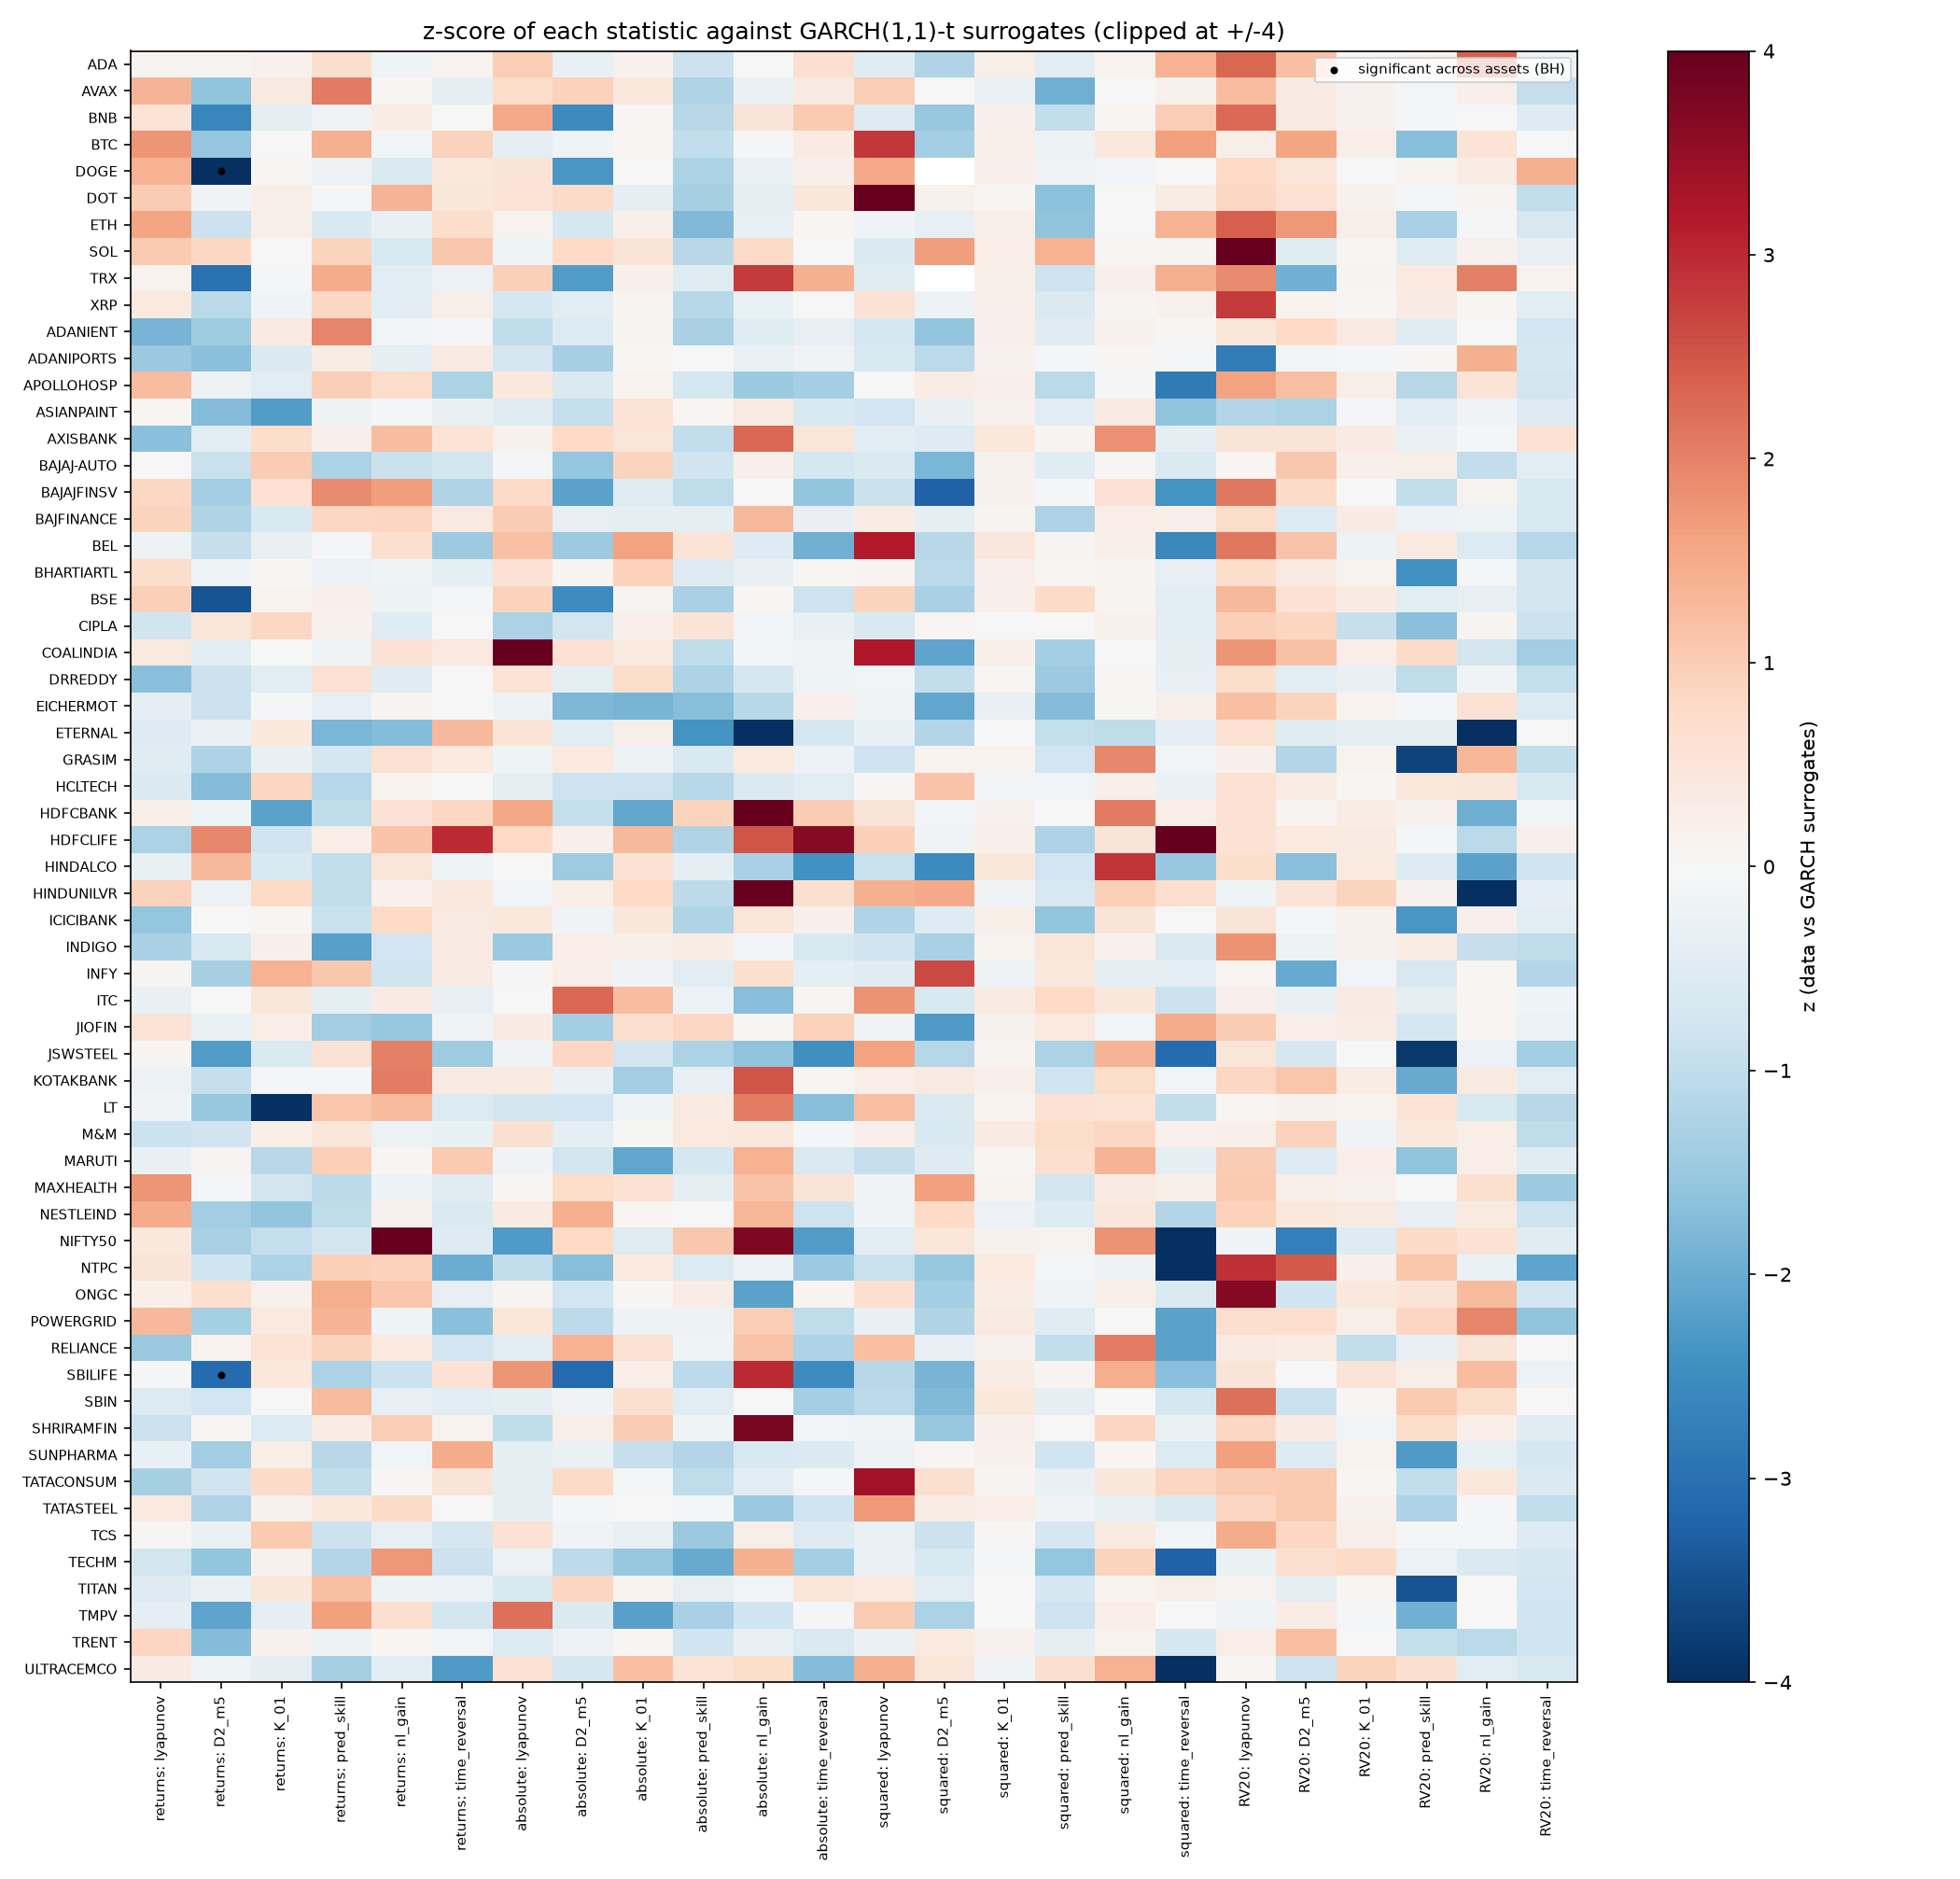
\includegraphics[width=\textwidth]{figures/01_z_vs_garch_heatmap.png}
\caption{Effect size $z$ of each statistic against GARCH(1,1)-$t$ surrogates for every asset (rows) and every series
and statistic (columns), clipped at $\pm 4$. Black dots mark the two tests that are significant after cross-asset
false discovery rate control.}
\label{fig:heat}
\end{figure}

Within assets, 13 of the 244 series have at least one statistic significant against GARCH after within-asset
correction (five cryptocurrency series and eight Nifty series), and all 13 are classified \emph{Inconclusive} because none
meets the conditions for a chaotic classification: in each case fewer than two deterministic statistics are
significant against both surrogate families, or $D_2$ does not saturate. Of these 13, three (BSE,
DOGE and HDFCLIFE) show the same departure in the first half of the sample and none in the second half. The final
classification is 231 series \emph{Random/Stochastic}, 13 \emph{Inconclusive}, and none \emph{Periodic},
\emph{Quasi-periodic} or \emph{Potentially Chaotic}.

\subsection{Power spectra of returns and volatility}

Return spectra are flat. The median spectral exponent of returns is 0.11 for cryptocurrencies and 0.03 for Nifty
series, with $R^2$ of 0.03 and 0.08, and the share of power at periods above 20 days, 0.09 in both markets, equals the
share expected for white noise. No whole-spectrum test against GARCH is significant across assets for any series in
either market, and no return series has a significant weekly component (smallest nominal $p$ 0.21 for crypto at
seven days and 0.021 for stocks at five days, neither significant after correction).

Volatility spectra rise steeply towards low frequencies, as expected for a persistent volatility process
(Figure~\ref{fig:btc} for Bitcoin). Table~\ref{tab:spec} reports the spectral summaries. For Nifty stocks the
spectral exponent of realised volatility (median 1.88) is almost identical to the median exponent of the GARCH
surrogates (1.86), and the observed exponent lies inside the 95\% surrogate range in 86\% of stocks. For
cryptocurrencies the exponent of realised volatility (median 1.60) is lower than that of the GARCH surrogates (2.28)
and lies below the 95\% surrogate range in seven of ten coins (Figure~\ref{fig:beta}); these differences reach
nominal significance in seven coins but do not survive cross-asset correction. The fitted GARCH models of
cryptocurrencies are close to integrated (for Bitcoin, $\alpha+\beta=1.000$ over the full sample), so the surrogates
are, if anything, \emph{more} persistent than the data. The low-band share tells the same story with stronger
evidence: after cross-asset correction, realised volatility of five cryptocurrencies (DOGE, ETH, SOL, TRX, XRP) has
\emph{less} power at periods above 20 days than its GARCH surrogates (median share 0.94 against 0.97), whereas squared
returns of 18 Nifty series (including the index) have \emph{more} (median 0.20 against 0.15). Volatility of the two
markets thus departs from GARCH(1,1) in opposite directions: cryptocurrency volatility is less persistent than an
integrated GARCH implies, and equity volatility contains more slow variation than a GARCH(1,1) captures.

\begin{table}[t]
\centering
\small
\caption{Spectral summaries (medians across assets). $\beta$: spectral exponent over periods 25--250 days;
$\beta_{\mathrm{G}}$: median exponent of the GARCH surrogates; GPH: Geweke--Porter-Hudak estimate of $\beta$; Low:
share of power at periods $>20$ days, data and GARCH surrogates. Weekly: number of assets with a significant
seven-day (crypto) or five-day (Nifty) component against GARCH after cross-asset correction.}
\label{tab:spec}
\begin{tabular}{llrrrrrrr}
\toprule
Market & Series & $\beta$ & $R^2$ & $\beta_{\mathrm{G}}$ & GPH & Low & Low$_{\mathrm{G}}$ & Weekly \\
\midrule
\multirow{4}{*}{Crypto (10)} & returns & 0.11 & 0.03 & 0.00 & 0.23 & 0.09 & 0.09 & 0/10\\
 & absolute returns & 0.45 & 0.23 & 1.03 & 0.86 & 0.22 & 0.27 & 10/10\\
 & squared returns & 0.19 & 0.17 & 0.74 & 0.52 & 0.15 & 0.20 & 0/10\\
 & realised vol (20d) & 1.60 & 0.77 & 2.28 & 0.97 & 0.94 & 0.97 & 5/10\\
\midrule
\multirow{4}{*}{Nifty (51)} & returns & 0.03 & 0.08 & 0.00 & $-0.09$ & 0.09 & 0.09 & 0/51\\
 & absolute returns & 0.70 & 0.61 & 0.61 & 0.64 & 0.20 & 0.17 & 0/51\\
 & squared returns & 0.71 & 0.69 & 0.52 & 0.45 & 0.20 & 0.15 & 0/51\\
 & realised vol (20d) & 1.88 & 0.84 & 1.86 & 0.75 & 0.95 & 0.95 & n.a.\\
\bottomrule
\end{tabular}
\end{table}

\begin{figure}[p]
\centering
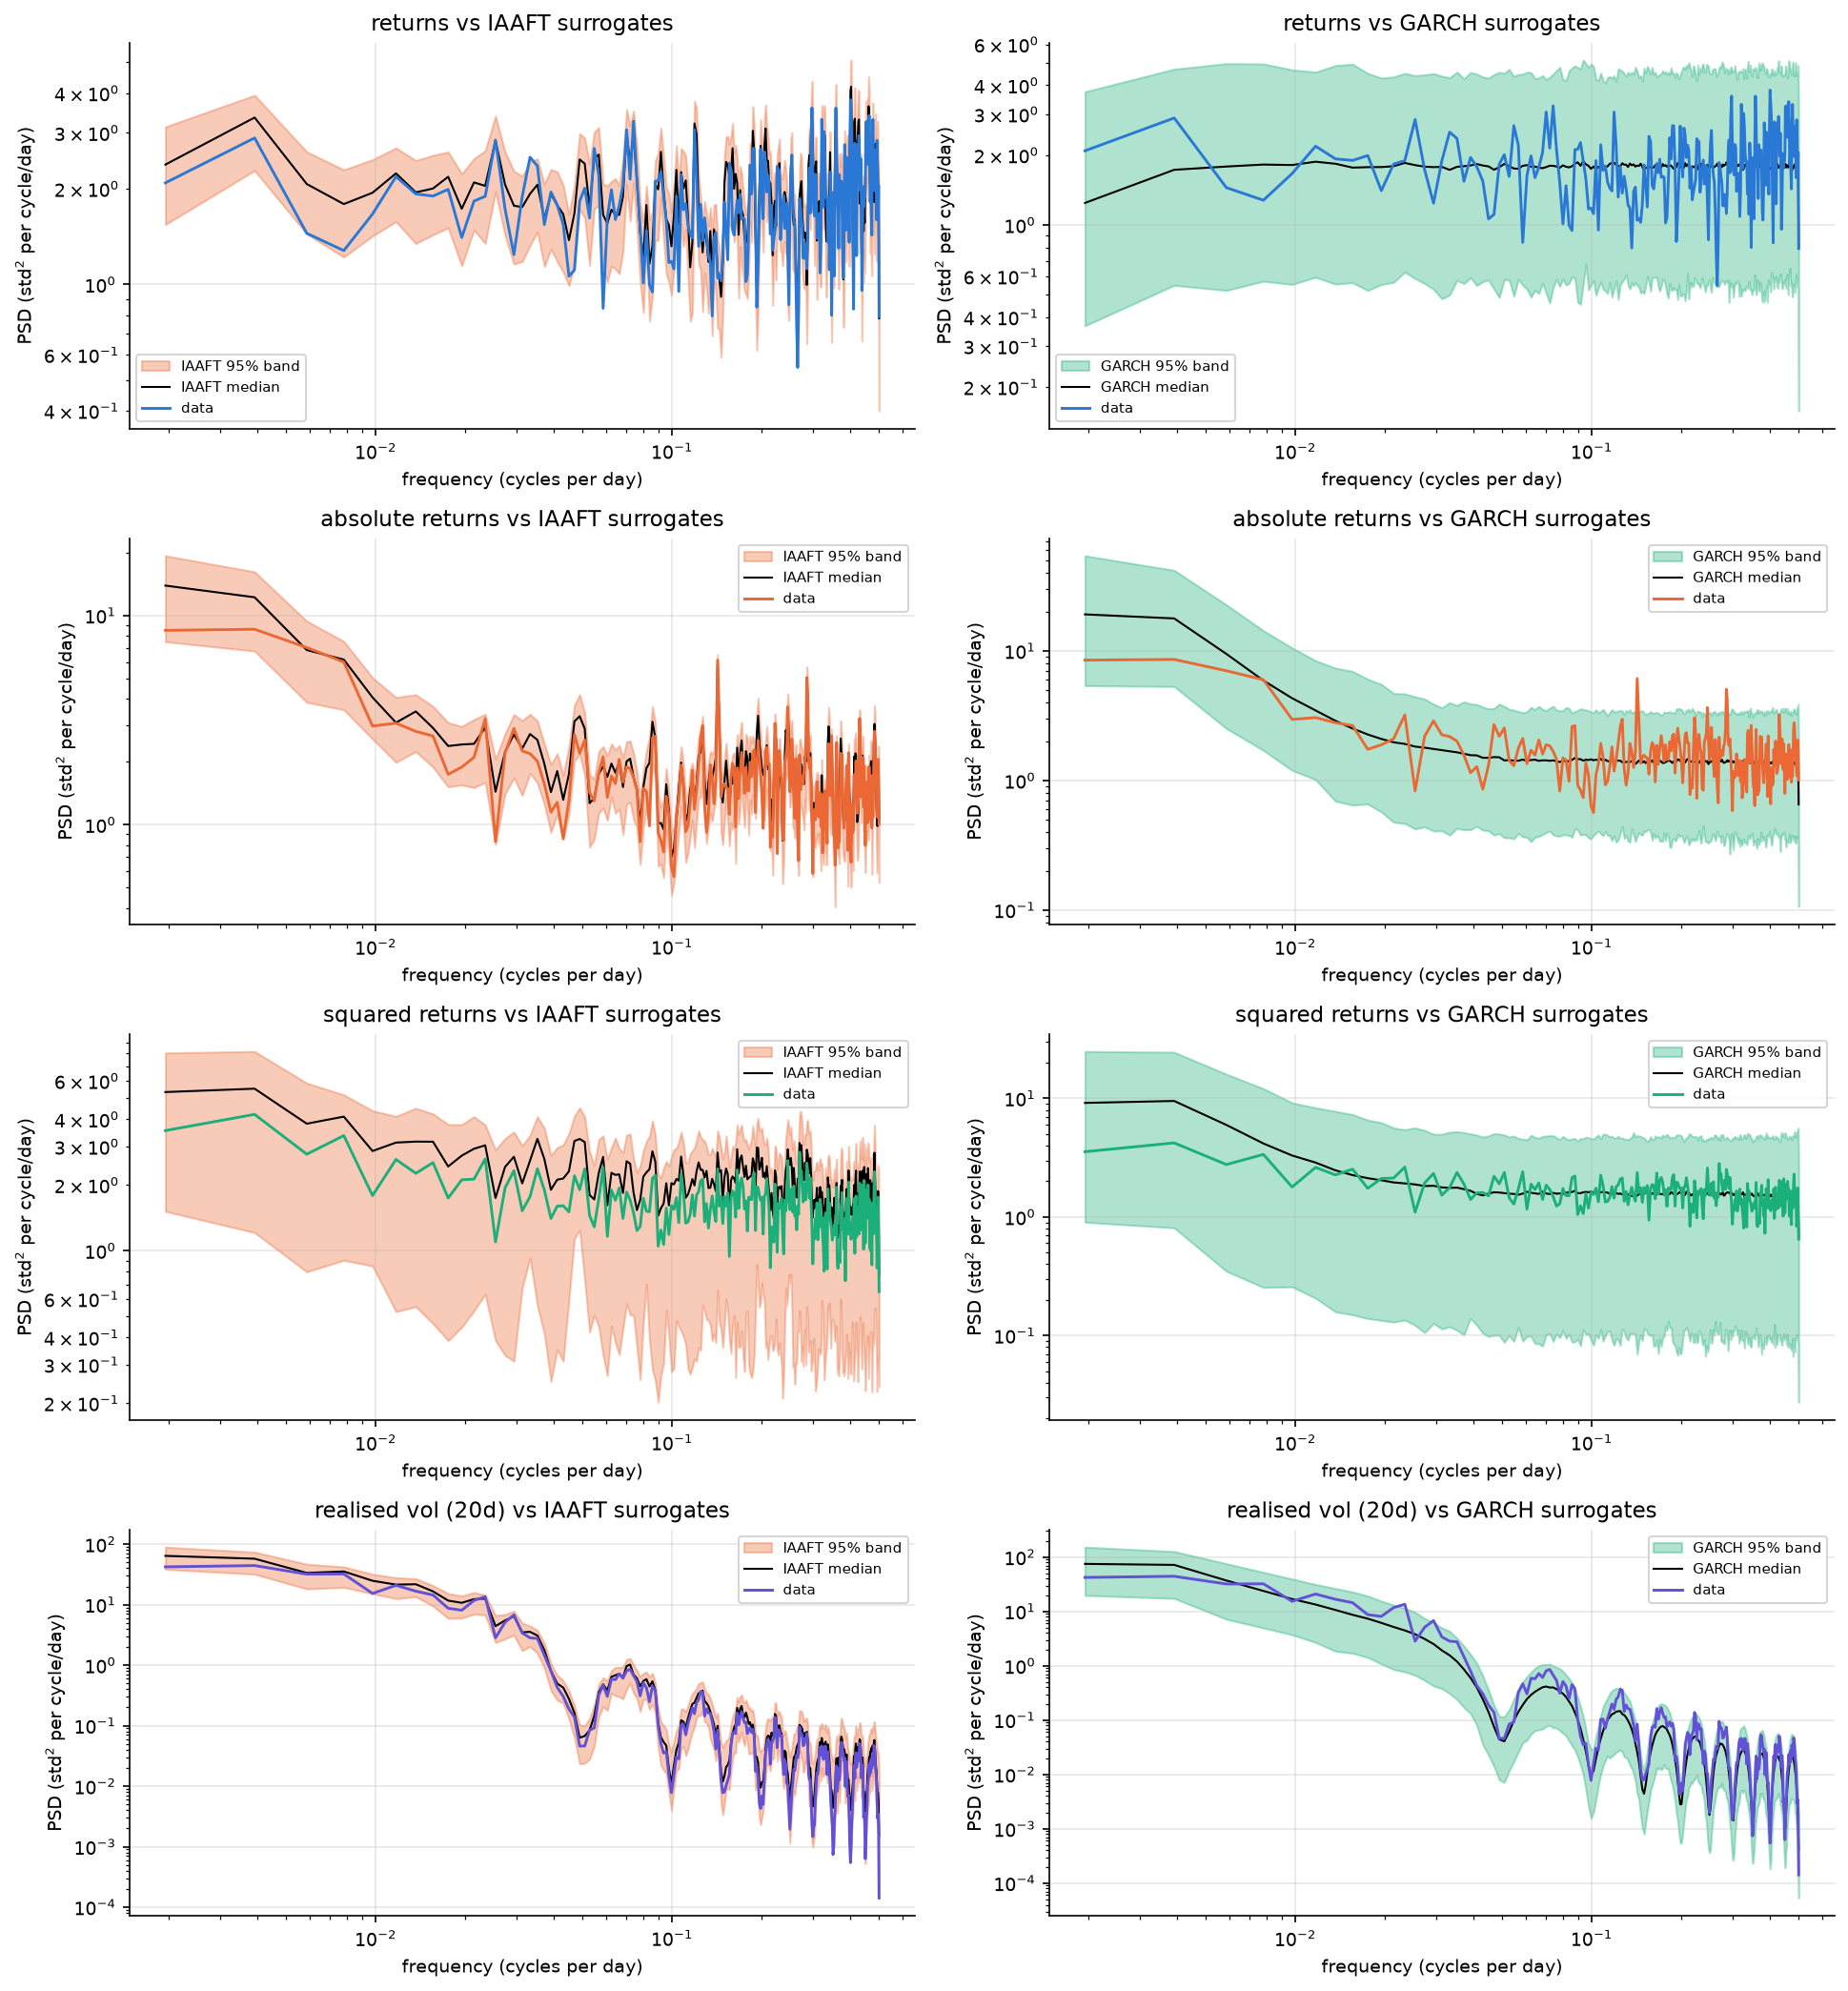
\includegraphics[width=0.92\textwidth]{figures/05_surrogate_spectra.png}
\caption{Bitcoin, full sample: Welch spectra of the four series (coloured) with the median (black) and 95\% band of 999
IAAFT surrogates (left) and 999 GARCH(1,1)-$t$ surrogates (right). The evenly spaced dips in realised volatility are
the zeros of the 20-day moving average at $f=k/20$.}
\label{fig:btc}
\end{figure}

\begin{figure}[t]
\centering
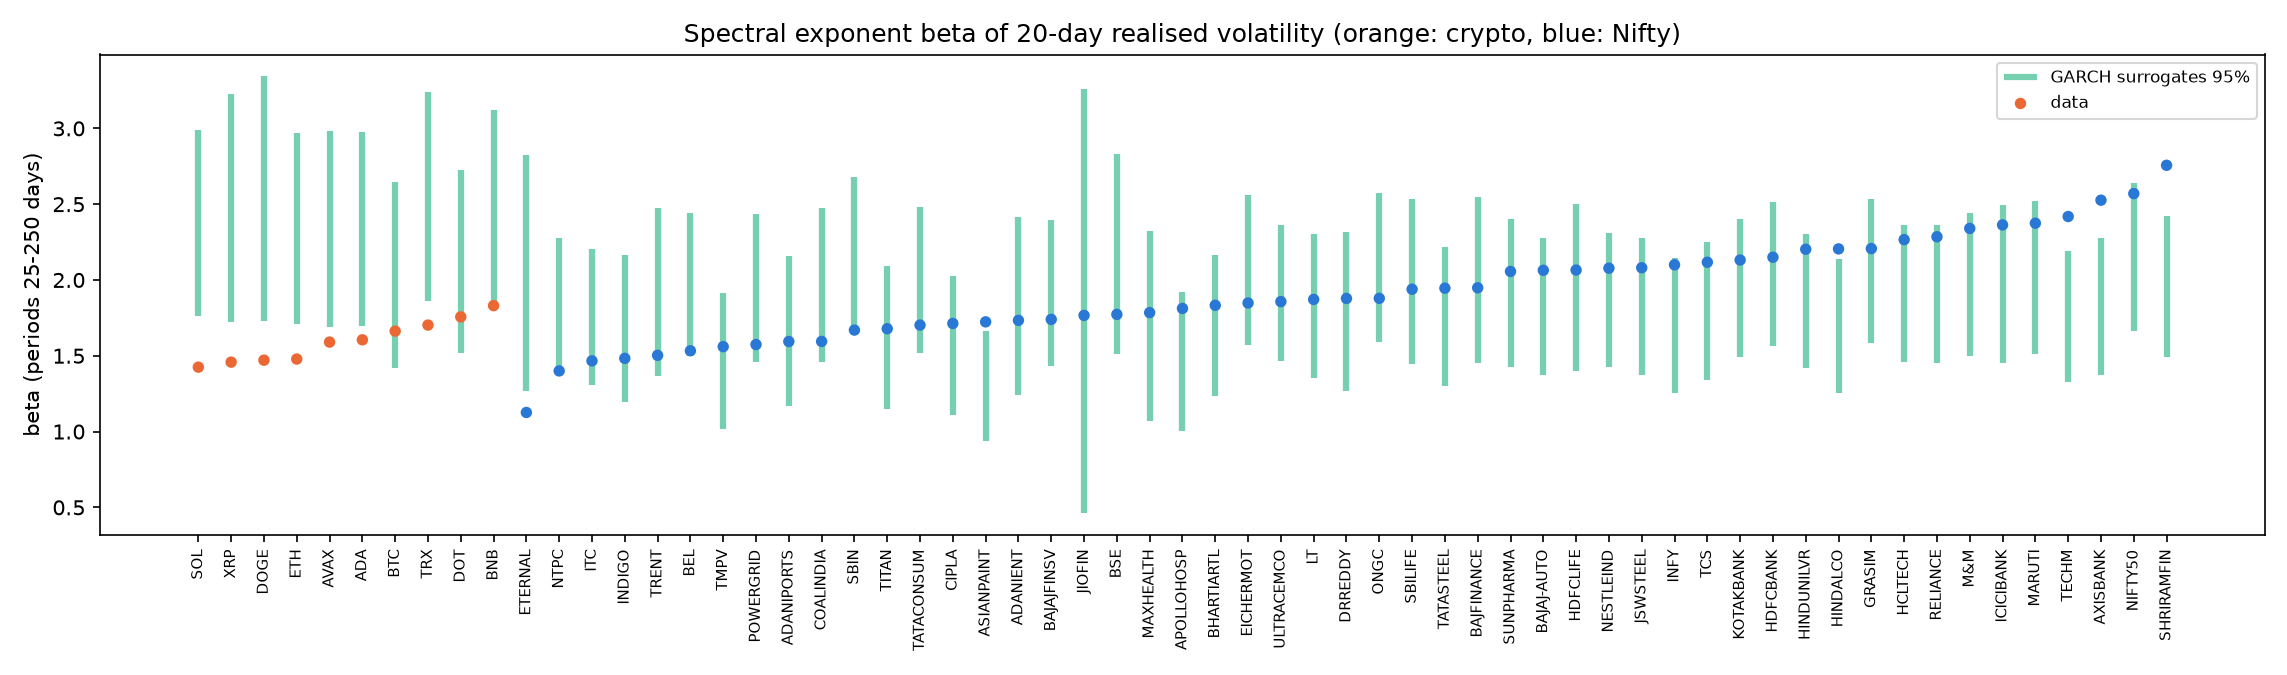
\includegraphics[width=\textwidth]{figures/02_beta_rv_by_asset.png}
\caption{Spectral exponent of 20-day realised volatility for every asset (dots; orange: cryptocurrencies, blue: Nifty)
with the 95\% range of the exponent over 999 GARCH(1,1)-$t$ surrogates of the same asset (bars).}
\label{fig:beta}
\end{figure}

\subsection{A weekly cycle in cryptocurrency volatility}

The only feature that departs from the GARCH null consistently across assets is a peak at a period of seven days in
cryptocurrency volatility. After cross-asset correction, the spectral power of absolute returns at seven days exceeds
the GARCH surrogate distribution in all ten cryptocurrencies (nominal $p$ between 0.001 and 0.017; cross-asset $q\le
0.017$), and that of realised volatility in five (ADA, AVAX, BTC, ETH and TRX). Squared returns show the same direction
with weaker evidence (nominal $p<0.05$ in two coins, none significant after correction), as expected for a statistic
dominated by a few extreme days. No Nifty series shows a significant five-day component in absolute or squared
returns. Because the effect is in volatility and not in returns, and is present in a market that trades every day of
the week but absent in one that is closed at weekends, the natural interpretation is a weekly pattern in trading
activity and volatility of the kind documented by \citet{Baur2019} and \citet{AharonQadan2019}. A GARCH(1,1) model
without day-of-week terms cannot generate such a pattern, which explains why it is the one feature the null misses.
It is a deterministic seasonal component of a stochastic volatility process, not evidence of chaotic dynamics.

\subsection{Market periods}

Volatility levels differ strongly across periods (Figure~\ref{fig:periods}). The median standard deviation of daily
cryptocurrency returns is 0.052, 0.068, 0.042 and 0.041 in P1 to P4, and the median excess kurtosis is 3.2, 13.7, 5.6 and
4.1; for Nifty series the corresponding values are 0.017, 0.023, 0.015 and 0.016, and 3.4, 7.3, 2.6 and 3.5. The
second period, which contains the COVID-19 crash, is the most volatile and most heavy-tailed in both markets. The
spectral \emph{shape}, however, changes little. The low-band share of realised volatility stays between 0.92 and 0.94
in crypto and between 0.89 and 0.95 in Nifty, and its spectral exponent between 1.60 and 1.92 in crypto; in Nifty it
is highest in P2 (2.45) and between 1.51 and 1.64 in the other periods. Against period-specific GARCH surrogates, 38 of
932 global spectral tests have nominal $p<0.05$, close to the 47 expected by chance; after cross-asset correction two
remain significant (absolute returns of HINDUNILVR and of the Nifty 50 index in 2016--2019), and no test on the
spectral exponent or the low-band share is significant. Within each period, therefore, the spectra are consistent
with a GARCH process refitted to that period: the regimes differ in the level and scale of volatility, not in the
type of dynamics.

\begin{figure}[t]
\centering
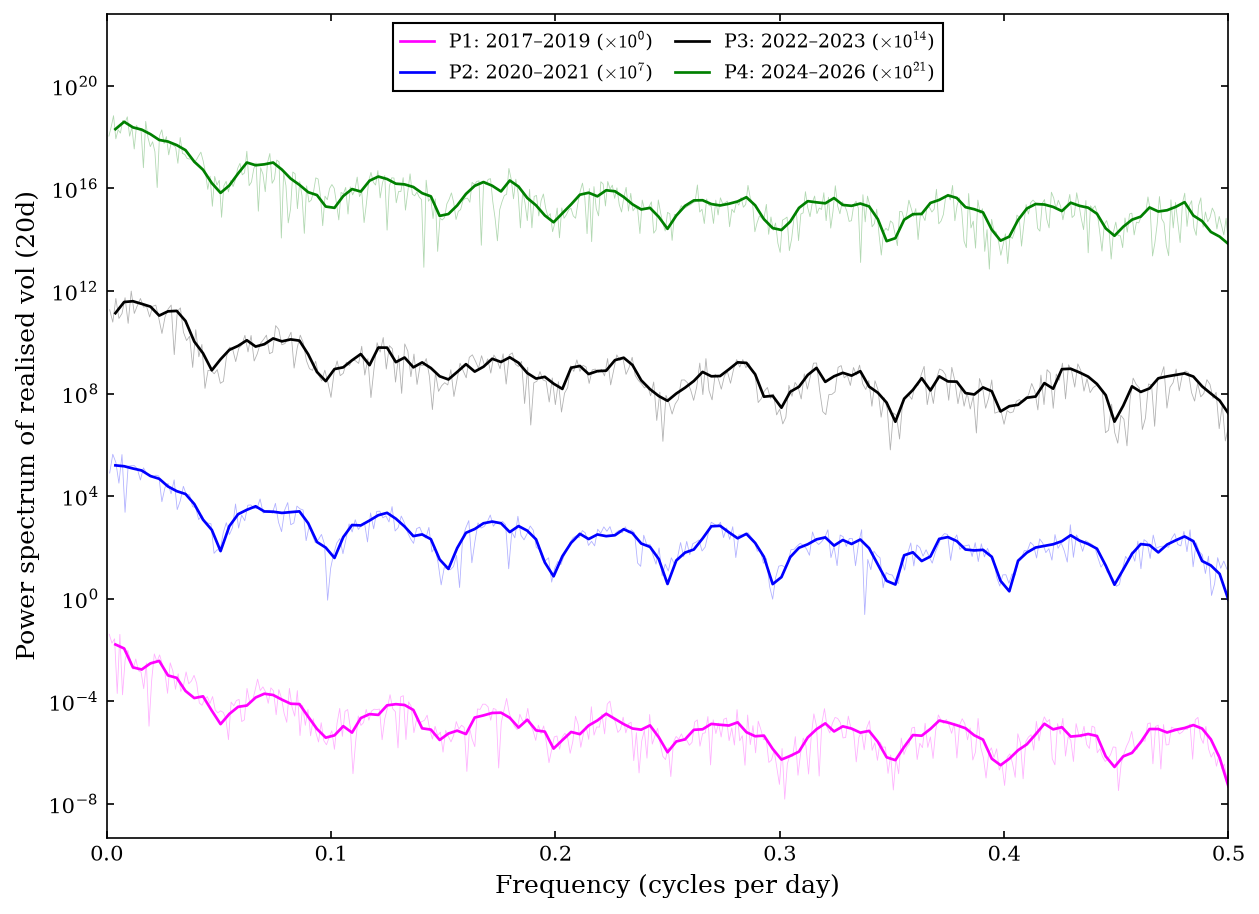
\includegraphics[width=0.62\textwidth]{figures/11_spectra_periods_realised_vol_20d.png}
\caption{Bitcoin: Welch spectra of 20-day realised volatility in the four market periods, offset vertically by
the stated factors for readability (log scale), in the style of \citet{KailashamKhair2023}.}
\label{fig:periods}
\end{figure}

\begin{figure}[t]
\centering
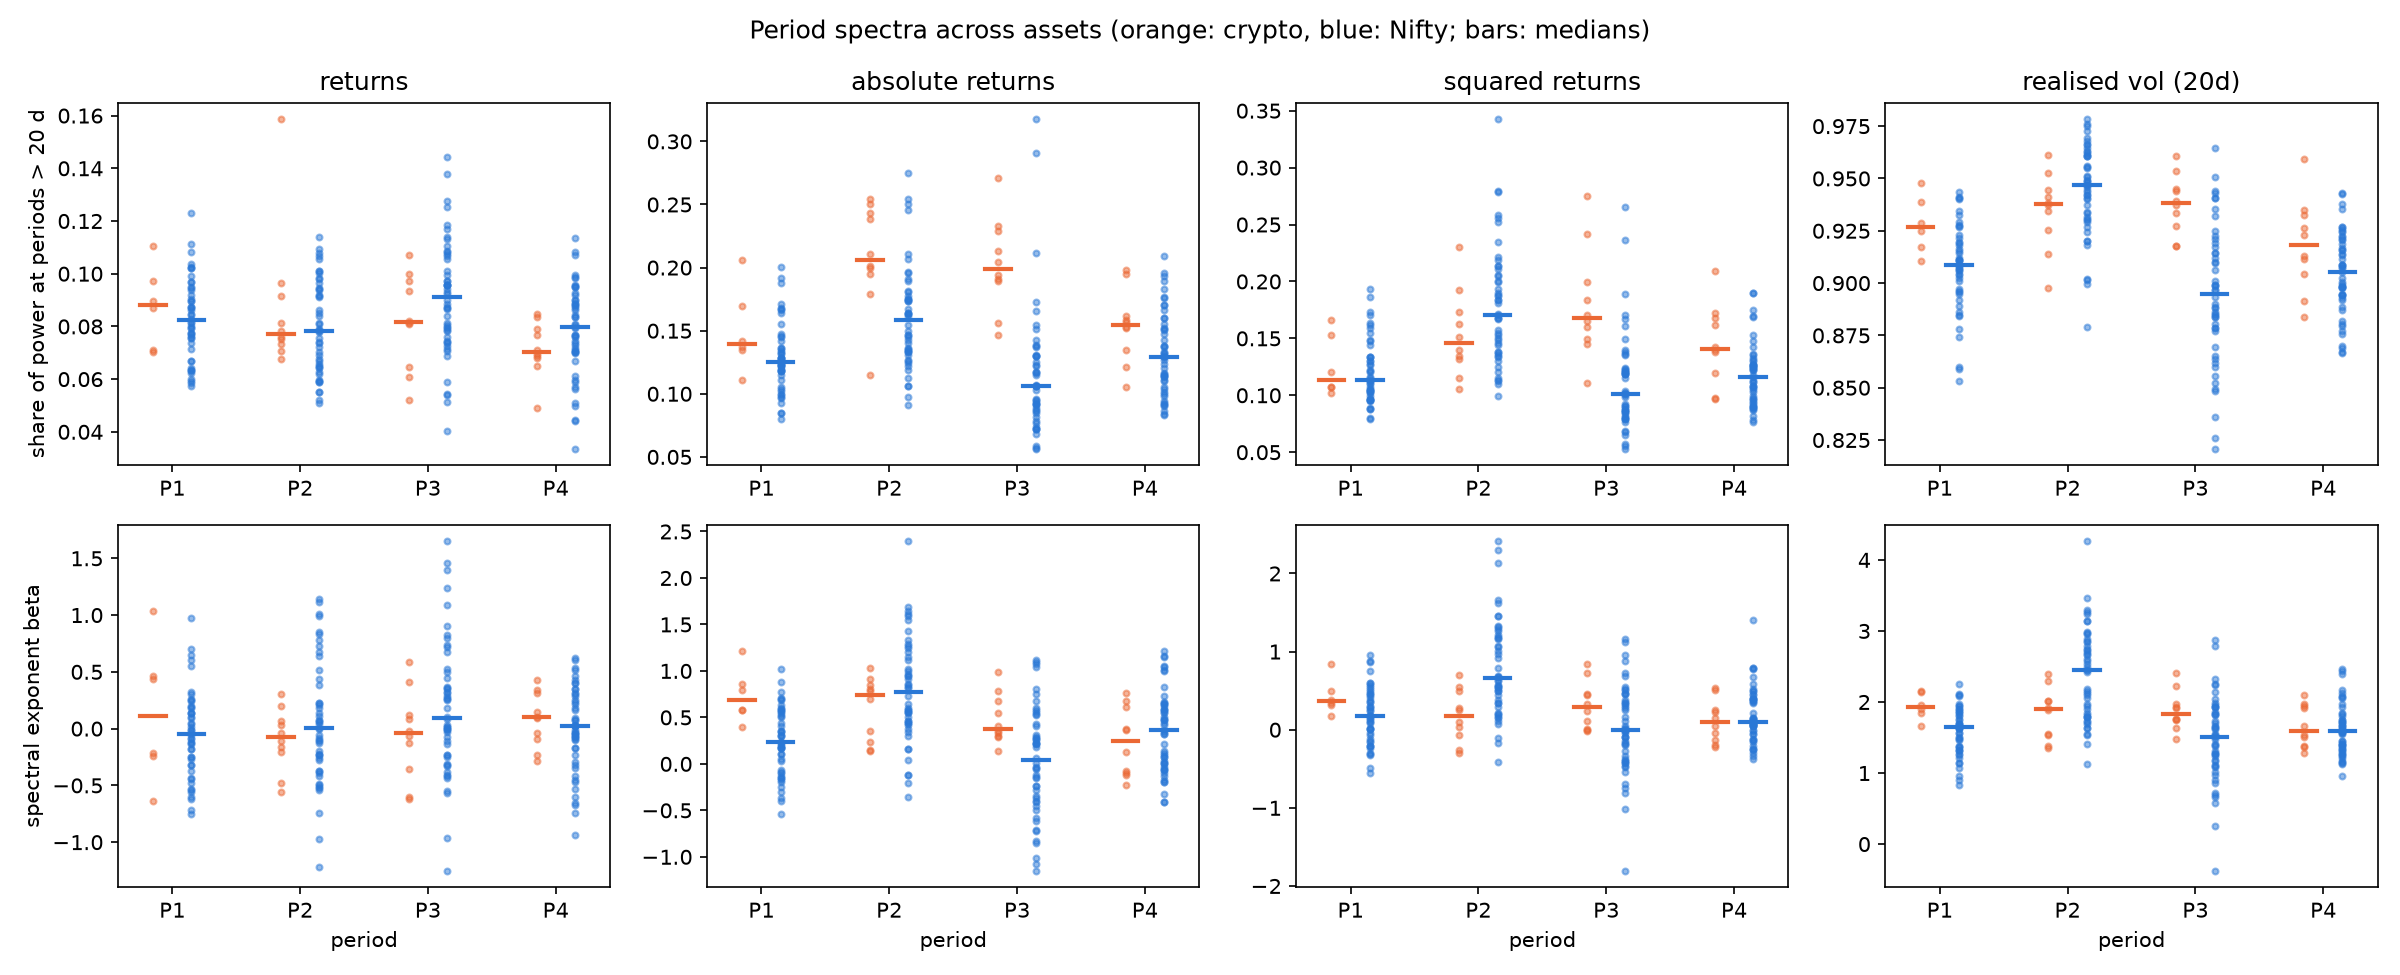
\includegraphics[width=\textwidth]{figures/04_period_spectra_across_assets.png}
\caption{Low-band share (top) and spectral exponent over periods 25--128 days (bottom) in the four market periods for
every asset (dots) with market medians (bars); orange: cryptocurrencies, blue: Nifty.}
\label{fig:periodsall}
\end{figure}

% ------------------------------------------------------------------------------------------------------------
\section{Discussion}\label{sec:discussion}

\subsection{What the evidence does and does not show}

The central result is that every conventional indicator of chaos (positive Lyapunov exponent, saturating
correlation dimension, $K\approx 1$) is present in these data and equally present in
series simulated from a GARCH(1,1)-$t$ model. These indicators therefore carry no information about determinism in
daily financial data, which confirms, on a larger and more homogeneous sample, the warnings of
\citet{OsborneProvenzale1989}, \citet{Ruelle1990} and \citet{Hsieh1991}. A study that reports chaos in a financial
series on the basis of a positive Lyapunov exponent alone, or against a linear or independent null only, is
reporting a property of volatility clustering.

The second result is that the null of a linear Gaussian process is rejected widely, and that this rejection is
almost entirely accounted for by GARCH. That the Lyapunov exponent of returns is \emph{lower} than in IAAFT surrogates
is consistent with this: clustering of large returns makes nearby states in the reconstructed space evolve more
similarly than in a linearised, phase-randomised version of the same series. The two significant departures from
GARCH after cross-asset correction are both correlation-dimension results, do not co-occur with any predictive
statistic and do not replicate across sample halves. We regard them as false positives or as artefacts of
misspecification of the GARCH tails, not as findings.

The third result is that the frequency domain is where the GARCH(1,1) null is most informatively wrong. In
cryptocurrencies it misses a weekly cycle in volatility and overstates low-frequency persistence; in Indian stocks it
understates the low-frequency power of squared returns in about a third of assets. The latter is consistent with the
long-memory and multi-component volatility literature \citep{DingGrangerEngle1993,Baillie1996,Corsi2009}, and with the
possibility that slowly changing volatility levels across regimes produce apparent long memory
\citep{LamoureuxLastrapes1990,MikoschStarica2004}; our period analysis, in which within-period spectra agree with
period-specific GARCH fits, supports the second explanation at least in part. The former is consistent with the
calendar evidence of \citet{Baur2019} and \citet{AharonQadan2019}, here confirmed for ten coins and shown to be the
main deficiency of a standard volatility model as a null for nonlinearity tests.

\subsection{Interpretation of the two markets}

Cryptocurrency and equity volatility differ in more than level. Cryptocurrency volatility shows positive time-reversal
asymmetry (increments skewed upwards, that is, sudden increases followed by gradual decreases), a weekly cycle and
less persistence than its near-integrated GARCH fit implies. Indian equity volatility shows more slow variation than a
GARCH(1,1) captures and, in most of the significant cases, time-reversal asymmetry of the opposite sign, whose
mechanism we leave for further work. None of these
differences involves deterministic dynamics; all are statements about the structure of a stochastic volatility process.
They nevertheless matter for practice: volatility models for cryptocurrencies should include calendar terms, and
models for equities may benefit from a slow volatility component.

% ------------------------------------------------------------------------------------------------------------
\section{Conclusion}\label{sec:conclusion}

Using a uniform protocol, two surrogate families and false discovery rate control across 61 assets, we find no
evidence of low-dimensional deterministic chaos in the daily returns or volatility of ten major cryptocurrencies or
of the Nifty 50 stocks and index. The usual indicators of chaos are reproduced by a GARCH(1,1)-$t$ model, the
widespread nonlinearity relative to a linear null is explained by conditional heteroskedasticity, and no series meets
the criteria for a chaotic classification. The departures from GARCH that do survive are spectral and have a clear
economic interpretation: a weekly cycle in cryptocurrency volatility, and market-specific differences in the
low-frequency persistence of volatility. Future work should calibrate the power of the protocol on synthetic chaotic
systems contaminated by realistic volatility noise, extend the null model to include calendar effects and long memory,
and examine intraday data, where the number of observations is large enough to give the diagnostics a fairer chance.

\section*{Data and code availability}
All results were produced with a single configuration file and fixed random seeds; per-asset tables, surrogate test
results and figures are stored with the analysis code. The data were obtained from public sources and were not
modified.

% ------------------------------------------------------------------------------------------------------------
\begin{thebibliography}{99}
\setlength{\itemsep}{2pt}
\small

\bibitem[Abhyankar et~al.(1997)]{Abhyankar1997}
Abhyankar, A., Copeland, L.S., Wong, W., 1997. Uncovering nonlinear structure in real-time stock-market indexes: the
S\&P 500, the DAX, the Nikkei 225, and the FTSE-100. \emph{Journal of Business \& Economic Statistics} 15, 1--14.

\bibitem[Aharon and Qadan(2019)]{AharonQadan2019}
Aharon, D.Y., Qadan, M., 2019. Bitcoin and the day-of-the-week effect. \emph{Finance Research Letters} 31, 415--424.

\bibitem[Andersen and Bollerslev(1997)]{AndersenBollerslev1997}
Andersen, T.G., Bollerslev, T., 1997. Intraday periodicity and volatility persistence in financial markets.
\emph{Journal of Empirical Finance} 4, 115--158.

\bibitem[Andersen et~al.(2003)]{Andersen2003}
Andersen, T.G., Bollerslev, T., Diebold, F.X., Labys, P., 2003. Modeling and forecasting realized volatility.
\emph{Econometrica} 71, 579--625.

\bibitem[Baillie et~al.(1996)]{Baillie1996}
Baillie, R.T., Bollerslev, T., Mikkelsen, H.O., 1996. Fractionally integrated generalized autoregressive conditional
heteroskedasticity. \emph{Journal of Econometrics} 74, 3--30.

\bibitem[Barnett and Serletis(2000)]{BarnettSerletis2000}
Barnett, W.A., Serletis, A., 2000. Martingales, nonlinearity, and chaos. \emph{Journal of Economic Dynamics and
Control} 24, 703--724.

\bibitem[Bariviera(2017)]{Bariviera2017}
Bariviera, A.F., 2017. The inefficiency of Bitcoin revisited: a dynamic approach. \emph{Economics Letters} 161, 1--4.

\bibitem[Baur et~al.(2019)]{Baur2019}
Baur, D.G., Cahill, D., Godfrey, K., Liu, Z.F., 2019. Bitcoin time-of-day, day-of-week and month-of-year effects in
returns and trading volume. \emph{Finance Research Letters} 31, 78--92.

\bibitem[Benjamini and Hochberg(1995)]{BenjaminiHochberg1995}
Benjamini, Y., Hochberg, Y., 1995. Controlling the false discovery rate: a practical and powerful approach to multiple
testing. \emph{Journal of the Royal Statistical Society B} 57, 289--300.

\bibitem[Bollerslev(1986)]{Bollerslev1986}
Bollerslev, T., 1986. Generalized autoregressive conditional heteroskedasticity. \emph{Journal of Econometrics} 31,
307--327.

\bibitem[Bollerslev(1987)]{Bollerslev1987}
Bollerslev, T., 1987. A conditionally heteroskedastic time series model for speculative prices and rates of return.
\emph{Review of Economics and Statistics} 69, 542--547.

\bibitem[Brock et~al.(1996)]{BDS1996}
Brock, W.A., Dechert, W.D., Scheinkman, J.A., LeBaron, B., 1996. A test for independence based on the correlation
dimension. \emph{Econometric Reviews} 15, 197--235.

\bibitem[Brock and Hommes(1998)]{BrockHommes1998}
Brock, W.A., Hommes, C.H., 1998. Heterogeneous beliefs and routes to chaos in a simple asset pricing model.
\emph{Journal of Economic Dynamics and Control} 22, 1235--1274.

\bibitem[Brock et~al.(1991)]{BrockHsiehLeBaron1991}
Brock, W.A., Hsieh, D.A., LeBaron, B., 1991. \emph{Nonlinear Dynamics, Chaos, and Instability: Statistical Theory and
Economic Evidence}. MIT Press, Cambridge, MA.

\bibitem[Caporale and Plastun(2019)]{Caporale2019}
Caporale, G.M., Plastun, A., 2019. The day of the week effect in the cryptocurrency market. \emph{Finance Research
Letters} 31, 258--269.

\bibitem[Cont(2001)]{Cont2001}
Cont, R., 2001. Empirical properties of asset returns: stylized facts and statistical issues. \emph{Quantitative
Finance} 1, 223--236.

\bibitem[Corbet et~al.(2019)]{Corbet2019}
Corbet, S., Lucey, B., Urquhart, A., Yarovaya, L., 2019. Cryptocurrencies as a financial asset: a systematic analysis.
\emph{International Review of Financial Analysis} 62, 182--199.

\bibitem[Corsi(2009)]{Corsi2009}
Corsi, F., 2009. A simple approximate long-memory model of realized volatility. \emph{Journal of Financial
Econometrics} 7, 174--196.

\bibitem[Diks et~al.(1995)]{Diks1995}
Diks, C., van Houwelingen, J.C., Takens, F., DeGoede, J., 1995. Reversibility as a criterion for discriminating time
series. \emph{Physics Letters A} 201, 221--228.

\bibitem[Ding et~al.(1993)]{DingGrangerEngle1993}
Ding, Z., Granger, C.W.J., Engle, R.F., 1993. A long memory property of stock market returns and a new model.
\emph{Journal of Empirical Finance} 1, 83--106.

\bibitem[Eckmann et~al.(1987)]{Eckmann1987}
Eckmann, J.-P., Kamphorst, S.O., Ruelle, D., 1987. Recurrence plots of dynamical systems. \emph{Europhysics Letters}
4, 973--977.

\bibitem[Eckmann and Ruelle(1985)]{EckmannRuelle1985}
Eckmann, J.-P., Ruelle, D., 1985. Ergodic theory of chaos and strange attractors. \emph{Reviews of Modern Physics}
57, 617--656.

\bibitem[Eckmann and Ruelle(1992)]{EckmannRuelle1992}
Eckmann, J.-P., Ruelle, D., 1992. Fundamental limitations for estimating dimensions and Lyapunov exponents in dynamical
systems. \emph{Physica D} 56, 185--187.

\bibitem[Engle(1982)]{Engle1982}
Engle, R.F., 1982. Autoregressive conditional heteroscedasticity with estimates of the variance of United Kingdom
inflation. \emph{Econometrica} 50, 987--1007.

\bibitem[Frank and Stengos(1989)]{FrankStengos1989}
Frank, M., Stengos, T., 1989. Measuring the strangeness of gold and silver rates of return. \emph{Review of Economic
Studies} 56, 553--567.

\bibitem[Fraser and Swinney(1986)]{FraserSwinney1986}
Fraser, A.M., Swinney, H.L., 1986. Independent coordinates for strange attractors from mutual information.
\emph{Physical Review A} 33, 1134--1140.

\bibitem[French(1980)]{French1980}
French, K.R., 1980. Stock returns and the weekend effect. \emph{Journal of Financial Economics} 8, 55--69.

\bibitem[Geweke and Porter-Hudak(1983)]{GewekePorterHudak1983}
Geweke, J., Porter-Hudak, S., 1983. The estimation and application of long memory time series models. \emph{Journal
of Time Series Analysis} 4, 221--238.

\bibitem[Gottwald and Melbourne(2004)]{GottwaldMelbourne2004}
Gottwald, G.A., Melbourne, I., 2004. A new test for chaos in deterministic systems. \emph{Proceedings of the Royal
Society of London A} 460, 603--611.

\bibitem[Gottwald and Melbourne(2009)]{GottwaldMelbourne2009}
Gottwald, G.A., Melbourne, I., 2009. On the implementation of the 0--1 test for chaos. \emph{SIAM Journal on Applied
Dynamical Systems} 8, 129--145.

\bibitem[Granger(1966)]{Granger1966}
Granger, C.W.J., 1966. The typical spectral shape of an economic variable. \emph{Econometrica} 34, 150--161.

\bibitem[Grassberger and Procaccia(1983)]{GrassbergerProcaccia1983}
Grassberger, P., Procaccia, I., 1983. Characterization of strange attractors. \emph{Physical Review Letters} 50,
346--349.

\bibitem[Harvey et~al.(2016)]{Harvey2016}
Harvey, C.R., Liu, Y., Zhu, H., 2016. \ldots and the cross-section of expected returns. \emph{Review of Financial
Studies} 29, 5--68.

\bibitem[Hinich(1982)]{Hinich1982}
Hinich, M.J., 1982. Testing for Gaussianity and linearity of a stationary time series. \emph{Journal of Time Series
Analysis} 3, 169--176.

\bibitem[Hsieh(1989)]{Hsieh1989}
Hsieh, D.A., 1989. Testing for nonlinear dependence in daily foreign exchange rates. \emph{Journal of Business} 62,
339--368.

\bibitem[Hsieh(1991)]{Hsieh1991}
Hsieh, D.A., 1991. Chaos and nonlinear dynamics: application to financial markets. \emph{Journal of Finance} 46,
1839--1877.

\bibitem[Kailasham and Khair(2023)]{KailashamKhair2023}
Kailasham, R., Khair, A.S., 2023. Non-Brownian diffusion and chaotic rheology of autophoretic disks. \emph{Physical
Review E} 107, 044609.

\bibitem[Kantz and Schreiber(2004)]{KantzSchreiber2004}
Kantz, H., Schreiber, T., 2004. \emph{Nonlinear Time Series Analysis}, 2nd ed. Cambridge University Press, Cambridge.

\bibitem[Katsiampa(2017)]{Katsiampa2017}
Katsiampa, P., 2017. Volatility estimation for Bitcoin: a comparison of GARCH models. \emph{Economics Letters} 158,
3--6.

\bibitem[Kennel et~al.(1992)]{Kennel1992}
Kennel, M.B., Brown, R., Abarbanel, H.D.I., 1992. Determining embedding dimension for phase-space reconstruction using a
geometrical construction. \emph{Physical Review A} 45, 3403--3411.

\bibitem[Kyrtsou and Serletis(2006)]{KyrtsouSerletis2006}
Kyrtsou, C., Serletis, A., 2006. Univariate tests for nonlinear structure. \emph{Journal of Macroeconomics} 28,
154--168.

\bibitem[Lahmiri and Bekiros(2018)]{LahmiriBekiros2018}
Lahmiri, S., Bekiros, S., 2018. Chaos, randomness and multi-fractality in Bitcoin market. \emph{Chaos, Solitons \&
Fractals} 106, 28--34.

\bibitem[Lamoureux and Lastrapes(1990)]{LamoureuxLastrapes1990}
Lamoureux, C.G., Lastrapes, W.D., 1990. Persistence in variance, structural change, and the GARCH model. \emph{Journal
of Business \& Economic Statistics} 8, 225--234.

\bibitem[Lancaster et~al.(2018)]{Lancaster2018}
Lancaster, G., Iatsenko, D., Pidde, A., Ticcinelli, V., Stefanovska, A., 2018. Surrogate data for hypothesis testing of
physical systems. \emph{Physics Reports} 748, 1--60.

\bibitem[Lo(1991)]{Lo1991}
Lo, A.W., 1991. Long-term memory in stock market prices. \emph{Econometrica} 59, 1279--1313.

\bibitem[Mandelbrot(1963)]{Mandelbrot1963}
Mandelbrot, B., 1963. The variation of certain speculative prices. \emph{Journal of Business} 36, 394--419.

\bibitem[Marwan et~al.(2007)]{Marwan2007}
Marwan, N., Romano, M.C., Thiel, M., Kurths, J., 2007. Recurrence plots for the analysis of complex systems.
\emph{Physics Reports} 438, 237--329.

\bibitem[Mayfield and Mizrach(1992)]{MayfieldMizrach1992}
Mayfield, E.S., Mizrach, B., 1992. On determining the dimension of real-time stock-price data. \emph{Journal of
Business \& Economic Statistics} 10, 367--374.

\bibitem[Mikosch and St\u{a}ric\u{a}(2004)]{MikoschStarica2004}
Mikosch, T., St\u{a}ric\u{a}, C., 2004. Nonstationarities in financial time series, the long-range dependence, and the
IGARCH effects. \emph{Review of Economics and Statistics} 86, 378--390.

\bibitem[Osborne and Provenzale(1989)]{OsborneProvenzale1989}
Osborne, A.R., Provenzale, A., 1989. Finite correlation dimension for stochastic systems with power-law spectra.
\emph{Physica D} 35, 357--381.

\bibitem[Peters(1991)]{Peters1991}
Peters, E.E., 1991. \emph{Chaos and Order in the Capital Markets}. Wiley, New York.

\bibitem[Ramsey and Rothman(1996)]{RamseyRothman1996}
Ramsey, J.B., Rothman, P., 1996. Time irreversibility and business cycle asymmetry. \emph{Journal of Money, Credit and
Banking} 28, 1--21.

\bibitem[Rosenstein et~al.(1993)]{Rosenstein1993}
Rosenstein, M.T., Collins, J.J., De Luca, C.J., 1993. A practical method for calculating largest Lyapunov exponents from
small data sets. \emph{Physica D} 65, 117--134.

\bibitem[Ruelle(1990)]{Ruelle1990}
Ruelle, D., 1990. Deterministic chaos: the science and the fiction. \emph{Proceedings of the Royal Society of London A}
427, 241--248.

\bibitem[Sauer et~al.(1991)]{Sauer1991}
Sauer, T., Yorke, J.A., Casdagli, M., 1991. Embedology. \emph{Journal of Statistical Physics} 65, 579--616.

\bibitem[Scheinkman and LeBaron(1989)]{ScheinkmanLeBaron1989}
Scheinkman, J.A., LeBaron, B., 1989. Nonlinear dynamics and stock returns. \emph{Journal of Business} 62, 311--337.

\bibitem[Schreiber and Schmitz(1996)]{SchreiberSchmitz1996}
Schreiber, T., Schmitz, A., 1996. Improved surrogate data for nonlinearity tests. \emph{Physical Review Letters} 77,
635--638.

\bibitem[Schreiber and Schmitz(2000)]{SchreiberSchmitz2000}
Schreiber, T., Schmitz, A., 2000. Surrogate time series. \emph{Physica D} 142, 346--382.

\bibitem[Sugihara(1994)]{Sugihara1994}
Sugihara, G., 1994. Nonlinear forecasting for the classification of natural time series. \emph{Philosophical
Transactions of the Royal Society of London A} 348, 477--495.

\bibitem[Sugihara and May(1990)]{SugiharaMay1990}
Sugihara, G., May, R.M., 1990. Nonlinear forecasting as a way of distinguishing chaos from measurement error in time
series. \emph{Nature} 344, 734--741.

\bibitem[Takens(1981)]{Takens1981}
Takens, F., 1981. Detecting strange attractors in turbulence. In: Rand, D.A., Young, L.-S. (Eds.), \emph{Dynamical
Systems and Turbulence, Warwick 1980}. Lecture Notes in Mathematics 898, Springer, Berlin, 366--381.

\bibitem[Theiler(1986)]{Theiler1986}
Theiler, J., 1986. Spurious dimension from correlation algorithms applied to limited time-series data. \emph{Physical
Review A} 34, 2427--2432.

\bibitem[Theiler et~al.(1992)]{Theiler1992}
Theiler, J., Eubank, S., Longtin, A., Galdrikian, B., Farmer, J.D., 1992. Testing for nonlinearity in time series: the
method of surrogate data. \emph{Physica D} 58, 77--94.

\bibitem[Tsay(1986)]{Tsay1986}
Tsay, R.S., 1986. Nonlinearity tests for time series. \emph{Biometrika} 73, 461--466.

\bibitem[Urquhart(2016)]{Urquhart2016}
Urquhart, A., 2016. The inefficiency of Bitcoin. \emph{Economics Letters} 148, 80--82.

\bibitem[Welch(1967)]{Welch1967}
Welch, P.D., 1967. The use of fast Fourier transform for the estimation of power spectra: a method based on time
averaging over short, modified periodograms. \emph{IEEE Transactions on Audio and Electroacoustics} 15, 70--73.

\bibitem[Wolf et~al.(1985)]{Wolf1985}
Wolf, A., Swift, J.B., Swinney, H.L., Vastano, J.A., 1985. Determining Lyapunov exponents from a time series.
\emph{Physica D} 16, 285--317.

\end{thebibliography}
\end{document}
